\chapter{Lokale Kurventheorie im euklidischen Raum}
\section{Grundbegriffe der Kurventheorie}
Wir betrachten zunächst (kurzzeitig) rein \uline{affingeometrische} Begriffe/Invarianten.
\begin{definition}
 Ein \uline{\(\C^r\)-Weg}\index{Weg} oder eine \uline{parametrisierte \(\C^r\)-Kurve}\index{Kurve} (\(r\ge 0\)) [\(\C^r = r\)-mal stetig differenzierbar] im (affinen) \(\IR^n\) ist eine \(\C^r\)-Abbildung 
\[
 c\colon t\in I \subset \IR \mapsto c(t)\in \IR^n
\]
eines offenen Intervalls \(I\) in den \(\IR^n\). \\
\(t\) heißt \uline{Parameter}\index{Parameter}, die Bildmenge \(c[I] \subset \IR^n\) die \uline{Spur des Weges}\index{Spur}. \\
Ein \(\C^r\)-Weg (\(r\ge 1\)) heißt \uline{regulär}\index{regulär}, wenn überall der \uline{Tangentenvektor}\index{Tangentenvektor} \(\dot c(t) = \frac{\dd c}{\dd t}(t) \ne 0\) ist. Nichtreguläre Punkte \(c(t_0)\) mit \(\dot c(t_0)=0\) heißen \uline{Singularitäten}\index{Singularität}.
\end{definition}
\begin{kin}
\(t \mapsto c(t)\) beschreibt die \uline{zeit}abhängige Bewegung eines Punktes im \(\IR^n\).
\(\dot c\) ist die vektorielle Geschwindigkeit\index{Geschwindigkeit} (und im euklidischen \(\IR^n\) \(w:= | \dot c|\) die skalare Geschwindigkeit).
\end{kin}
\begin{bsp}\(\)
\begin{enumerate}
 \item \uline{Peano-Kurve}: Stetiger (\(\C^0\)-)Weg im \(\IR^2\), dessen Spur jeden Punkt eines Gebietes \(G\subseteq \IR^2\) ausfüllt (nirgends differenzierbar, "`unbrauchbar"')
 \item \uline{Konstanter Weg}: \(t \in I \mapsto c(t)=x_0 \in \IR^n\) (nirgends regulär, "`unbrauchbar"')
 \item \uline{Neil'sche Parabel}: \(c \colon t\in \IR \mapsto c(t) = \begin{pmatrix}
                                                                t^2 \\
								t^3
                                                               \end{pmatrix}
								\in \IR^2 \)\quad (\(\C^\infty\)-Weg), in \(c(0)=\begin{pmatrix}
								                                                  0 \\
														  0
								                                                 \end{pmatrix} \) nicht regulär ("`Spitze"') (\(w(0)=|\dot c (0)|=0\), "`man hat Zeit, sich umzudrehen"')
 \item \uline{Kreislinie}: \(c\colon t\in \IR \mapsto c(t)=\begin{pmatrix}
                                                       \cos t \\
						       \sin t
                                                      \end{pmatrix} \in \IR^2\) ( \(\infty\)-oft durchlaufbar) [Affin gesehen ist das eine Ellipse!] \\
Aber auch \(t \mapsto \widetilde c(t) = \begin{pmatrix}
                                     t \\
				     \pm \sqrt{1-t^2}
                                    \end{pmatrix} \) und \(t \mapsto \widetilde{\widetilde c}(t)=\begin{pmatrix}
											  \frac{1}{\cosh t} \\
											  \tanh t
											 \end{pmatrix} \)
sind Parametrisierungen von Kreisstücken.
\end{enumerate}
\end{bsp}
Wege,  die nur mit veränderlicher "`Zeitskala"' durchlaufen werden, sollen nicht als verschieden angesehen werden.
\begin{definition}
 \(I, \widetilde I \subset \IR\) seien offene Intervalle. \\
Zwei Wege \(c \colon I \to \IR^n, \widetilde c \colon \widetilde I \to \IR^n\) heißen \uline{\(C^r\)-äquivalent}\index{Äquivalenz} (\(r\ge 0 \)), wenn ein orientierungstreuer\index{orientierungstreu} (d.h. monoton wachsender) \(\C^r\)-Diffeomorphismus\index{Diffeomorphismus} \(\Phi \colon I \to \widetilde I\) existiert, mit
\[
 \uline{c= \widetilde c \circ \Phi}, \text{ d.h. } \uline{\forall_t c(t)=\widetilde c (\Phi(t))}
\]

\end{definition}

\begin{bemerkung} \(\)
 \begin{enumerate}
  \item[0.] \(\Phi \, \C^r\)-Diffeomorphismus\index{Diffeomorphismus} \(\Leftrightarrow \Phi\) bijektiv und \(\Phi\) \uline{und \(\Phi^{-1}\)}\, \(C^r\)-differenzierbar. 
  [Bsp.: \(\Phi \colon t \in \IR \to t^3 \in \IR\) ist \uline{kein} \(\C^1\)-Diffeomorphismus] \\
  Bei \(C^r\)-Diffeomorphismus ist stets \(\dot \Phi(t)\ne 0\) (falls \(r\ge 1\))
  \item[1.] \(\Phi\) ist (für \(r\ge 1\)) genau dann orientierungstreu, wenn überall \(\dot \Phi(t)>0\) ist.
  \item[2.] Äquivalente Wege besitzen (für \(r\ge 1\)) das gleiche Regularitätsverhalten.
  \[
   \dot c(t)= \dot{\widetilde c} (\Phi(t)) \cdot \underbrace{\dot \Phi(t)}_{>0}
  \]
  \item[3.] Die Äquivalenz von Wegen ist wirklich eine Äquivalenzrelation (reflexiv, symmetrisch, transitiv)
 \end{enumerate}
\end{bemerkung}

\begin{definition}
 Eine (orientierte, reguläre) \uline{\(\C^r\)-Kurve} (\(r\ge1\)) im (affinen) \(\IR^n\) ist eine Äquivalenz-klasse \([c]\) von regulären \(\C^r\)-Wegen \(c \colon I \subset \IR \to \IR^n\). Ein Repräsentant heißt eine (zulässige) \uline{Parametrisierungen}\index{Parametrisierung} der \(\C^r\)-Kurve, eine die Äquivalenz vermittelnde Abbildung \(\Phi\) eine (zulässige) \uline{Parametertransformation}\index{Parametertransformation}.
\end{definition}

\begin{bsp}
 Die "`Kreis"'-Darstellungen\index{Kreis} 
 \[
 t \mapsto c(t)=\begin{pmatrix}
                 \cos t \\
                 \sin t
                \end{pmatrix} \in \IR^2, \left(|t|<\frac\pi2\right)
 \]
 und 
     \[
      \widetilde t\mapsto \widetilde c(\widetilde t) = \begin{pmatrix}
                                             \frac1{\cosh \widetilde t} \\
                                             \tanh \widetilde t
                                            \end{pmatrix} \in \IR^2 (\widetilde t \in \IR) 
     \]
 sind \(\C^\infty\)-äquivalente Parametertransformationen: \[
                                                            \Phi(t) = \operatorname{Artanh} \sin t = \widetilde t
                                                           \]
mit
\[
 \dot \Phi(t)=\frac{\cos t}{1-\sin^2 t}= \frac1{\cos t} >0
\]
\end{bsp}

\begin{bemerkung}
 Nicht jedes 1-dimensionale "`Gebilde"' im \(\IR^n\) (z.B. eine vollständige Kreislinie) lässt sich global und injektiv als Bild eines offenen Intervalls darstellen. \\
 Objekte, die sich nur lokal so parametrisieren lassen, heißen (1-dimensionale) differenzierbare Mannigfaltigkeiten\index{Mannigfaltigkeit}. Für lokale Untersuchungen ist eine solche Erweiterung der Kurvenbegriffs nicht nötig.
\end{bemerkung}

Die bisher eingeführten Begriffe sind offensichtlich affin-invariant. Aber im Folgenden sind auch nur Eigenschaften von \uline{Kurven} von Interesse, also Eigenschaften, die nicht von der Parametrisierung abhängen. \\
Hier ein Beispiel aus der rein affinen Differentialgeometrie. 
\begin{bsp}\(\)
\begin{figure}[ht]
 \centering
 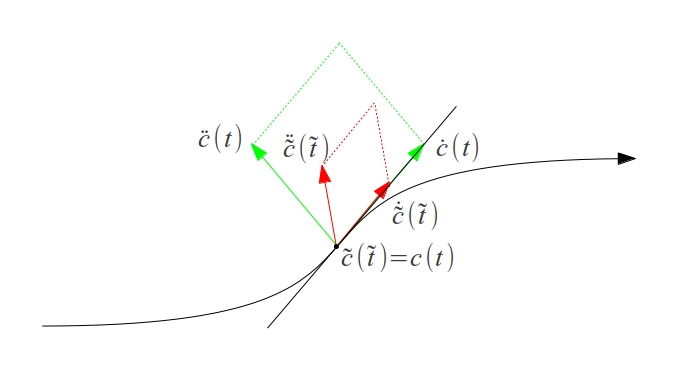
\includegraphics[width=11cm, height=5.5cm]{Bilder/Bsp1.jpg}
\end{figure} 
\end{bsp}

\begin{satz}\label{satz111}
 \(t \mapsto c(t)\) sei Parameterdarstellung einer \(\C^r\)-Kurve im (affinen) \(\IR^n\) mit \(r \ge n\). Dann sind die Ableitungsvektoren\index{Ableitungsvektor} 
 \[
  c_p:= \frac{\dd^p c}{\dd t^p} \, (p=1,\dots, n)
 \]
\uline{nicht} invariant gegenüber Parametertransformationen, jedoch die (punktualen, orientierten) \uline{Schmieg}-\uline{räume}\index{Schmiegraum} (oskulierende Räume, "`osculating spaces"') 
\[
 S_p(t):= c(t) + \langle \langle c_1(t), \dots , c_p(t) \rangle \rangle
\]
Spezialfälle: \\
Tangente \(S_1(t)=c(t) + \langle \langle \dot c(t) \rangle \rangle \) \\
Schmiegebene \( S_2(t) c(t) + \langle \langle \dot c(t), \ddot c(t) \rangle \rangle \)
\end{satz}

\begin{beweis}[von Satz \ref{satz111}]
 Aus \(c = \widetilde c \circ \Phi\) folgt nach der Kettenregel
 \begin{align*}
  \dot c &= \dot \Phi \left(\dot{\widetilde c} \circ \Phi \right)\\
  \ddot c &= \dot \Phi^2 \left( \ddot{\widetilde c} \circ \Phi \right) + Q_2^1 \left( \dot \Phi, \ddot \Phi \right) \cdot \dot {\widetilde c}(t)
 \end{align*}
allgemein 
\begin{align*}
 c_p= \dot \Phi^p (\widetilde c_p \circ \Phi) + \sum_{k=1}^{p-1} \underbrace{Q_p^k \left( \dot \Phi, \ddot \Phi \right)}_{\text{"`Kettenregelpolynome"'}} \left( \widetilde c_k \circ \Phi \right)
\end{align*}
Also hat man die Transformationsformel
\begin{align*}
 \begin{pmatrix}
  c_1 \\
  \vdots \\
  \vdots \\
  c_p
 \end{pmatrix} = \begin{pmatrix}
		  \dot \Phi &0 & \cdots & 0 \\
		  Q_2^1& \dot \Phi^2 & \ddots  & \vdots \\
		  \vdots & \ddots & \ddots &0 \\
		  Q_p^1 & \cdots & Q_p^k & \dot \Phi^p
		 \end{pmatrix} \begin{pmatrix}
				\widetilde c_1 \circ \Phi \\
				\vdots \\
				\vdots \\
				\widetilde c_p \circ \Phi
			       \end{pmatrix}
\end{align*}
mit einer regulären Transformationsmatrix positiver Determinante. \\
Das zeigt 
\[
 \langle \langle c_1, \dots, c_p \rangle \rangle = \langle \langle \widetilde c_1 \circ \Phi, \dots, \widetilde c_p \circ \Phi \rangle \rangle
\]
und die weiteren Behauptungen.
\end{beweis}

\begin{bemerkung}
 Die Regularitätsforderung \(\dot c(t) \ne 0\) bedeutet, dass in jedem Punkt die Tangenten als 1-dimensionale Unterräume existieren.
\end{bemerkung}

Die Schmiegräume kann man dazu benutzen, um festzustellen, ob eine Kurve in einem echten affinen Teilraum \(U_p \subset \IR^n\) liegt, in einer Geraden, einer Ebene usw. (affin-invariant!) \\
Zunächst gilt offensichtlich 
\[
 S_1(t) \subseteq S_2(t) \subseteq \dots \subseteq S_n(t) \le p
\]

\begin{satz}\label{satz112} \(\)
 \begin{enumerate}
  \item[a)] Liegt eine \(\C^{p+1}\)-Kurve in einem \(p\)-dimensionalen affinen Unterraum des \(\IR^n\) (\(1 \le p \le n-1 \)), so ist
  \[
   \forall_t \dim S_{p+1}(t) < p+1
  \]
  d.h. der (\(p+1\))-te Schmiegraum degeneriert\index{Schmiegraum!degeneriert}.
  \item[b)] Gilt umgekehrt 
  \[
   \forall_t \dim S_{p+1}(t) = \dim S_p(t) \stackrel{!}{=} p
  \]
  so liegt die Kurve in einem \(p\)-dimensionalen, aber keinem niedriger dimensionalen affinen Unterraum.
 \end{enumerate}
\end{satz}

\begin{anwendung} \(\)
 \begin{enumerate}
  \item Eine \(\C^2\)-Kurve \([c]\) im \(\IR^n\) verläuft genau dann \uline{geradlinig}, wenn \(\forall_t \big(\dot c(t), \ddot c(t)\big) \) linear abhängig ist. \\
  \big["`\(\Rightarrow\)"' nach a), "`\(\Leftarrow\)"' nach b), da \([c]\) regulär\big]
 \end{enumerate}
 \begin{definition}
  Ein (regulärer) Kurvenpunkt \(c(t)\) heißt \uline{Wendepunkt}\index{Wendepunkt} (WP, inflection point), falls \(\big(\dot c(t), \ddot c(t)\big)\) linear abhängig ist.
 \end{definition}
 \begin{enumerate}
  \item[2.] Eine \uline{wendepunktfreie}\index{Wendepunkt!-frei} \(\C^3\)-Kurve \([c]\) im \(\IR^n\) verläuft genau dann \uline{in einer Ebene}, wenn \\ 
  \(\forall_t \big( \dot c(t), \ddot c(t), \dddot c(t) \big) \) linear abhängig ist.
 \end{enumerate}
 \begin{definition}
  Ein \uline{Nicht-Wendepunkt}\index{Nicht-Wendepunkt} \(c(t)\) heißt "`\uline{Henkelpunkt}"'\index{Henkelpunkt} (handle point), wenn \( \big( \dot c(t), \ddot c(t), \dddot c(t) \big) \) linear abhängig ist.
 \end{definition}

\end{anwendung}

\begin{beweis}[von Satz \ref{satz112}] \(\)
 \begin{enumerate}
  \item[a)]
  \begin{align*}
   &\forall_t \quad c(t) = p_0 + \sum_{k=1}^p \lambda_k(t) \cdot a_k \in U_p = p_0 + \hl a_1, \dots, a_p \hr \Rightarrow \\
   &\overset{p+1}{\underset{l=1}\forall} \forall_t \quad c_l(t)= c^{(l)}(t) = \sum_{k=1}^p \lambda_k^{(l)}(t)\cdot a_k \in \hl a_1, \dots, a_p \hr \Rightarrow \\
   & \forall_t \quad \dim S_{p+1}(t) \le p < p
  \end{align*}
  \item[b)] Nach Voraussetzung ist \((c_1, \dots, c_p)(t) \) linear unabhängig, aber \((c_1, \dots, c_{p+1})(t) \) linear abhängig. Es existieren also Funktionen \(t \mapsto \lambda_0(t), \dots, \lambda_{p-1}(t)\) mit 
  \begin{align*}
   c_{p+1} = \sum_{k=1}^p \lambda_{k-1} c_k \text{ bzw. } \uline{(\dot c)^{(p)} = \sum_{k=0}^{p-1} \lambda_k (\dot c)^k} \tag{\(\ast\)}
  \end{align*}
  Die Funktionen sind stetig auf \(I\), denn \((\ast)\) kann nach \(\lambda_0, \dots, \lambda_{p-1}\) aufgelöst werden (Inhomogenes lineares Gleichungssystem mit vollrangiger Koeffizientenmatrix, da \(c_1, \dots, c_p\) linear unabhängig; Einträge und "`rechte Seite"' stetig). \\
  Die Koeffizientenfunktionen \(t \mapsto \dot c^{\,i}(t) \, (i=1,\dots, n)\) genügen also der linearen Differentialgleichung \(p\)-ter Ordnung
  \[
   y^{(p)} = \sum_{k=0}^{p-1} \lambda_k y^{(k)}
  \]
  mit stetigen Koeffizienten.
  für sie existiert ein Fundamentalsystem \(y_1, \dots y_p \colon I \to \IR\), so dass für jede Lösung gilt
  \[
   y(t)=\sum_{k=1}^p a_k y_k(t)
  \]
  also auch
  \[
   \dot c^{\,i}(t)=\sum_{k=1}^p a_k^i y_k(t)
  \]
  und damit
  \[
   \dot c(t)=\sum_{k=1}^p y_k(t) a_k
  \]
  mit konstanten Vektoren \(a_1, \dots, a_p \in \IR^n\). \\
  Integration liefert \(\forall_{t \in I}\)
  \[
   c(t)= c(t_0) + \sum_{k=1}^p \left(\int_{t_0}^t y_k(\tau) \dd \tau \right) a_k \in c(t_0) + \hl a_1, \dots, a_p \hr =: U_p
  \]
  Es ist schließlich 
  \[
  \uline{\dim U_p =p}
  \] 
  denn aus \(\dim U_p = k < p\) folgt nach a), dass \( \dim S_{k+1} < k+1 \), also auch \(\dim S_p <p\) im Widerspruch zur Voraussetzung.
 \end{enumerate}
  
\end{beweis}

Ab jetzt arbeiten wir im orientierten, \uline{euklidischen} Raum. Hier gibt es zum Glück in jeder Äqui\-va\-lenzklasse von Wegen einen ausgezeichneten Repräsentanten, die \uline{Bogenlängenparametrisierung} (kurz: BLP).

\begin{satz}\label{satz113}
 Sei \(t \mapsto c(t)\) Parameterdarstellung einer \(\C^1\)-Kurve im euklidischen\index{euklidisch} \(\IR^n\). Dann gibt es (bis auf eine additive Konstante) genau eine zulässige Parametertransformation 
 \[
  t \mapsto s(t) = \int|\dot c (t)| \dd t \, [+ s_0]
 \]
 (genannt Bogenlängenfunktion)\index{Bogenlängenfunktion}, so dass in der neuen Bogenlängenparametrisierung\index{Bogenlängenparametrisierung}
 \(
  \overline c = c \circ s^{-1}
 \)
 gilt
 \[
 \uline{|\overline c' | = 1}
 \]
 Die Konstruktion ist unabhängig von der Ausgangsparametrisierung.
\end{satz}

\begin{kin}
In Bogenlängenparametrisierung wird die Kurve mit konstanter Geschwindigkeit \(w = |\overline c'| \equiv 1\) durchlaufen ("`Zeit \(=\) Weg"'). Solche Wege heißen auch normal\index{normal}.
\end{kin}

\begin{beweis}[von Satz \ref{satz113}]
 Für die gesuchte Transformation \(s\) muss wegen 
 \[
 c = \overline c \circ s \Rightarrow |\dot c| = \underbrace{|\overline c' \circ s|}_{= 1} \underbrace{\dot s}_{> 0}
 \]
 gelten: 
 \[
 \dot s = |\dot c|
 \]
Eine Stammfunktion 
 \[
 s = \int |\dot c|
 \]
leistet das Gewünschte, da sie \(\C^1\)-differenzierbar ist, mit 
\(
\dot s = |\dot c| > 0
\)
(wegen der Regularität von \(c\)). \\
 Für eine äquivalente Parametrisierung \(\widetilde c\) mit \(c = \widetilde c \circ \Phi\) der Kurve erhält man
 \[
  \dot s = |\dot c| = |\dot{\widetilde c} \circ \Phi| \underbrace{\dot \Phi}_{> 0} = (\widetilde s \circ \Phi) \cdot \dot \Phi
 \]
 also gilt 
 \[s = \widetilde s \circ \Phi \, (+ s_0)\] 
 und damit \[\overline c = c \circ s^{-1} = (\widetilde c \circ \Phi) \circ (\widetilde s \circ \Phi)^{-1} = \widetilde c \circ \Phi \circ \Phi^{-1} \circ \widetilde s^{-1} = \widetilde c \circ \widetilde s^{-1} = \overline{\widetilde c}\]
\end{beweis}

\begin{bemerkung}
 Mit der Bogenlängenfunktion \(t \mapsto s(t)\) kann man die \uline{Länge}\index{Weg!-länge} eines \(\C^1\)-Wegstücks \\
 \(t \in [a,b] \subset I \mapsto c(t) \in \IR^n\) messen.
 \[
  L_a^b(c) = s(b) - s(a) = \int_a^b |\dot c(t)| \dd t
 \]
 Diese erhält man aus den Längen einbeschriebener Polygonzüge durch Verfeinern und Grenzüber\-gänge. \(\C^1\)-Wege sind rektifizierbar.
\end{bemerkung}

\textbf{\uline{Praktische Berechnung der Bogenlängenparametrisierung}}\index{Bogenlängenparametrisierung!Berechnung} (Schreibweise schlampig): 
\begin{enumerate}
 \item Man berechne \mat{s = s(t) = \int |\dot c(t)| \dd t}
 \item bilde die Umkehrfunktkion \(t=t(s)\)
 \item und bilde \(c(s) = c\big(t(s)\big)\)
\end{enumerate}

\Links

\begin{bsp}
 Ellipse\index{Ellipse} \(t \mapsto c(t) = \vxy{a \cos t}{b \sin t}\) im \(\IR^2\) mit Halbachsen \(0 < a < b\)
 \begin{align*}
  \frac{\dd s}{\dd t}(t) &= |\dot c(t)| = \sqrt{a^2 \sin^2 t + b^2 \cos^2 t} \\
  &= b \cdot \sqrt{1 - \left[1-\left(\frac ab\right)^2\right] \sin^2 t} = b \cdot \sqrt{1-k^2 \sin^2 t} \\
  \Rightarrow s(t) &= b \cdot E(k,t) \, [+ s_0] \quad \text{(Elliptisches Integral 2. Gattung, nicht elementar integrierbar)}
 \end{align*}
 Für einen Kreis (\(a = b = r\)) gilt \(k = 0\) also
 \begin{align*}
  s &= s(t)=r \cdot t \tag {1.}\\
  t &= t(s) = \frac sr \quad \text{also} \tag {2.}\\
  c(s) &= \vxy{r \cos \frac sr}{r \sin \frac sr} \tag {3.}
 \end{align*}
\end{bsp}

\textbf{\uline{Ergebnis}:} \\
Bei Verwendung der Bogenlängenparametrisierung erhält man zwar immer sofort Größen, die invariant gegenüber Parametertransformationen sind.\\
\uline{Aber} meist lässt sie sich nicht explizit bestimmen und ist nur für theoretische Zwecke brauchbar. \\
\uline{Ausweg}: siehe später \\\\
Allgemein zu \uline{Bezeichnungen} (schlampig, aber praktisch)
\begin{center}
\begin{tabular}{c||c|c}
 & bei bel. Par.-Darst. & in BLP \\
 \hline
 \hline
 Parameter & \(t\) [Zeit] & \(s\) [Weg] \\
 \hline
 Parameterdarstellung & \(t \mapsto c(t)\) & \(s \mapsto c(s)\) \\
 \hline
 Ableitungen & \(\dot c, \ddot c, \dddot c, \dots\) [Zeitabl.] & \(c', c'', c''', \dots\) [Abl. nach BL] 
\end{tabular} 
\end{center}
Es gilt 
\[
 \dot c = c' \circ \dot s, \ddot c = c'' \cdot \dot s^2 + c' \ddot s, \dots
\]

\section{Kurven in der euklidischen Ebene $\IR^2$}
siehe Übungen
\section{Kurven im euklidischen Raum $\IR^3$}
\uline{Vorgehensweise} (in jeder Kurven- und Flächentheorie): \\
Konstruktion einer (möglichst invarianten) \uline{Begleitbasis} der Kurve ("`moving frame"'). Ihre \uline{Ableitungs}-\uline{gleichungen} liefern Invarianten für die Kurve, u.a. ihre \uline{Krümmungen}.

\subsection{FRENET-Begleitbasis, Krümmung und Torsion}
Die \uline{Krümmung}\index{Krümmung} einer Raumkurve in Bogenlängenparametrisierung \(s \mapsto c(s)\) soll deren Abweichung vom \uline{geradlinigen Verlauf} messen. Diese wird bestimmt durch die Änderung des (invarianten) Tangenteneinheitsvektors\index{Tangenteneinheitsvektor}
\[
T := c' = \frac{\dd c}{\dd s}
\]
\begin{satz}\label{satz131}
Für die \uline{Krümmung}\index{Krümmung}
\[
 s \mapsto \kappa(s) := |T'(s)| = |c''(s)| \ge 0
\]
einer \(\C^2\)-Kurve in Bogenlängenparametrisierung \(s \mapsto c(s)\) gilt
\begin{enumerate}
 \item[a)] \(\kappa(s_0)=0 \, \Leftrightarrow \,c(s_0)\) Wendepunkt
 \item[b)] \(\kappa \equiv 0 \, \Leftrightarrow\) die Kurve verläuft geradlinig
\end{enumerate}
\end{satz}

\begin{beweis}[von Satz \ref{satz131}] \(\)
 \begin{enumerate}
  \item[a)] \(\kappa(s_0) = 0 \, \Leftrightarrow \, T'(s_0) = 0 {{\color{red}\Leftarrow} \atop \Rightarrow} (c', c'')(s_0) = (T, T')(s_0)\) linear abhängig \\
  \(\Leftrightarrow \, c(s_0)\) ist Wendepunkt \\
  Für die {\color{red}Rückrichtung} wird benötigt: \\
   \[|T|^2 = \langle T,T\rangle = 1 \Rightarrow 2 \langle T',T\rangle = 0 \Rightarrow T' \perp T\] \\
   also \((T,T')(s_0)\) linear abhängig \(\Rightarrow T'(s_0)=0\)
   \item[b)] nach Satz \ref{satz112}, Anwendung 1 oder direkt
   \[
    \kappa \equiv 0 \Leftrightarrow T'= c'' = 0 \Leftrightarrow c(s) = x_0 + s \cdot X
   \]
 \end{enumerate}
\end{beweis}
Noch ein \uline{Test}, ob der Name "`Krümmung"' gerechtfertigt ist: \\
Für einen \uline{Kreis} in Bogenlängenparametrisierung \(s \mapsto c(s) = r \vxyz{\cos \frac sr}{\sin \frac sr}{0}\) im \(\IR^3\) gilt
\begin{align*}
 T(s) &= \vxyz{-\sin \frac sr}{\cos \frac sr}{0} \\
 T'(s) &= \frac 1r \vxyz{-\cos \frac sr}{-\sin \frac sr}{0} \\
 \kappa(s) &= \frac 1r
\end{align*}

\begin{satz}\label{satz132}
 Sei \(s \mapsto c(s)\) Bogenlängenparametrisierung einer \uline{wendepunktfreien} \(\C^2\)-Kurve im orientierten, euklidischen \(\IR^3\). Dann bilden die Vektorfelder
 \begin{align*}
  &s \mapsto T(s) := c'(s) & \text{[Tangentenvektor]} \\
  &s \mapsto H(s) := \frac{T'(s)}{|T'(s)|} & \text{[Hauptnormalenvektor]} \\
  &s \mapsto B(s) := (T \times H)(s) & \text{[Binormalenvektor]}
 \end{align*}\index{Hauptnormalenvektor}\index{Tangentenvektor}\index{Binormalenvektor}
 eine orthonormierte, positiv orientierte \(\C^0\)-Begleitbasis der Kurve, genannt \uline{\textsc{Frenet}-Begleitbasis}\index{Frenet-Begleitbasis}.
\end{satz}

\begin{beweis}[von Satz \ref{satz132}]
 \begin{align*}
  T'\perp T, T' \ne 0 \Rightarrow H \text{ definiert; Rest klar}
 \end{align*}

\end{beweis}

\begin{figure}[ht]
 \centering
 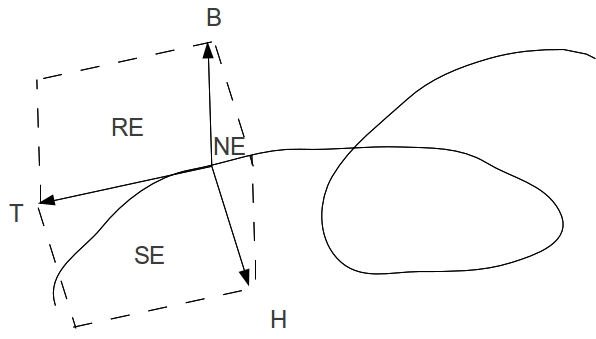
\includegraphics[scale=0.3]{Bilder/Bsp2.jpg}
\end{figure}

\begin{folgerung}
 In jedem Kurvenpunkt \(c(s)\) hat man die paarweise orthogonalen \uline{Begleitebenen}\index{Begleitebene}
 \begin{align*}
  &c(s) + \hl T,H \hr(s) \quad \big(\perp B(s)\big) & \text{[Schmiegebene]} \\
  &c(s) + \hl H,B \hr(s) \quad \big(\perp T(s)\big) & \text{[Normalebene]} \\
  &c(s) + \hl B,T \hr(s) \quad \big(\perp H(s)\big) & \text{[rektifizierende Ebene]} 
 \end{align*}\index{Schmiegebene}\index{Normalebene}\index{rektifizierende Ebene}
\end{folgerung}

Die \uline{Torsion}\index{Torsion} (Windung\index{Windung}, \uline{2. Krümmung}\index{Krümmung!2. Krümmung}) einer wendepunktfreien \(\C^3\)-Kurve (\(\Rightarrow (T,H,B) \C^1\)-differen\-zier\-bar) soll deren Abweichung vom ebenen Verlauf messen. Diese wird bestimmt durch die Änder\-ung des Binormalenvektors \(B\) (\(=\) Normalenvektor der Schmiegebene). \\
Wegen \(\begin{Bmatrix}
         B^2 = 1 & \Rightarrow \langle B,B'\rangle = 0  &\Rightarrow B' \perp B \\
         B = T \times H & \Rightarrow B' = \underbrace{T' \times H}_{= 0} + T \times H' &\Rightarrow B' \perp T
        \end{Bmatrix}\) gilt \\
        \(B' = -\tau H\) mit einer \(\C^0\)-Funktion
        \[
         \tau = -\langle B', H\rangle
        \]
        
\begin{satz}\label{satz133}
 Für die durch \(B' = - \tau H\) definierte \uline{Torsion}\index{Torsion} 
 \[
  s \mapsto \tau(s) = - \langle B', H \rangle (s) \stackrel{H \perp B}{=} + \langle H', B \rangle (s) \stackrel{B = T \times H}{=} \det (T,H,H')(s)
 \]
einer \uline{wendepunktfreien} \(\C^3\)-Kurve in Bogenlängenparametrisierung \(s \mapsto c(s)\) gilt
\begin{enumerate}
 \item[a)] \( \tau(s_0) = 0 \Leftrightarrow c(s)\) Henkelpunkt \(\Leftrightarrow \begin{Bmatrix}
                                                                                  (c', c'', c''')(s_0) &\text{linear abhängig} \\
                                                                                  (c',c'') (s_0) & \text{linear unabhängig}
                                                                                 \end{Bmatrix}\)
 \item[b)] \(\tau \equiv 0 \Leftrightarrow\) die Kurve verläuft eben.
\end{enumerate}
\end{satz}

\begin{beweis}[von Satz \ref{satz133}] \(\)
 \begin{enumerate}
  \item[a)] Allgemein gilt
  \begin{align*}
  \langle X \times Y, Z \rangle &= \sum_i (X \times Y)^i Z^i = \sum_{i=1}^3 \det (X,Y,e_i) Z^i \\
  &=\det(X,Y,Z)
  \end{align*}
  Darau folgt
  \begin{align*}
   \tau(s_0) &= \det (T,H,H')(s_0) = \det \left( c', \frac{c''}{\kappa}, \left(\frac{c''}{\kappa}\right)'\right)(s_0) \\
   &= \det \left(c', \frac{c''}{\kappa}, \left(\frac1\kappa\right)' c'' + \frac1\kappa c'''\right)(s_0) = \frac{1}{\kappa^2(s_0)} \det \left(c',c'',c'''\right)(s_0)=0
  \end{align*}
\(\Rightarrow (c', c'', c''')(s_0)\) linear abhängig
  \item[b)] Nach Satz \ref{satz112}, Anwendung 2
 \end{enumerate}
\end{beweis}

\begin{satz}\label{satz134}
 Für die Frenet-Begleitbasis \(s \mapsto (T,H,B)(s)\) einer wendepunktfreien \(\C^3\)-Kurve gelten die Frenetschen \uline{Ableitungsgleichungen}\index{Frenet-Begleitbasis!Ableitungsgleichungen}
 \[\begin{Bmatrix}
  T' &= &&\kappa H \\
  H' &= &-\kappa T &&+ \tau B \\
  B' &= &&-\tau H
 \end{Bmatrix} \text{bzw.}
 {\vxyz{T}{H}{B}}' = \begin{pmatrix}
                      0 & \kappa & 0 \\
                      -\kappa & 0 & \tau \\
                      0 & -\tau & 0
                     \end{pmatrix} \vxyz{T}{H}{B}
 \]
mit der \(\C^1\)-Krümmung \(s \mapsto \kappa(s) > 0\) und der \(\C^0\)-Torsion \(s \mapsto \tau(s) \).
\end{satz}

\begin{beweis}[von Satz \ref{satz134}] 
Da \((T_1, T_2, T_3) := (T,H,B)\) ein \uline{Orthonormalbasisfeld}\index{Orthonormalbasis!-feld} ist, gilt \(\langle T_i, T_k \rangle = \delta_{ik}\) \\
 \(\Rightarrow \langle T_i', T_k \rangle = -\langle T_k', T_i \rangle\), d.h. die Ableitungsmatrix\index{Ableitungsmatrix!$\IR^3$} \((\langle T_i', T_k \rangle)_{i,k=1,2,3}\) ist \uline{schiefsymmetrisch}. Damit kann die nach Definition bekannte 1. und 3. Zeile ergänzt werden.
\end{beweis}

\uline{Problem}: Wie berechnet man Begleitbasis, Krümmung und Torsion, wenn man die Bogenlängen\-parametrisierung nicht explizit kennt? \\
\uline{Lösung}: "`Rücktransformation"'

\begin{folgerung}
 Bezüglich einer beliebigen Parametrisierung \(t \mapsto c(t)\) einer wendepunktfreien \(\C^3\)-Kurve gilt
 \begin{align*}
  T &= \frac{\dot c}{|\dot c|} \\
  B &= \frac{\dot c \times \ddot c}{|\dot c \times \ddot c|} \\
  H &= B \times T = \frac{\ddot c - \langle \ddot c, T \rangle T}{|\ddot c - \langle \ddot c, T \rangle T|} \\
  \kappa &= \frac{|\dot c \times \ddot c|}{|\dot c|^3} \\
  \tau &= \frac{\det (\dot c, \ddot c, \dddot c)}{|\dot c \times \ddot c|^2}
 \end{align*}\index{Begleitbasis!Berechnung (unbekannte BLP)}\index{Krümmung!Berechnung (unbekannte BLP)}\index{Torsion!Berechnung (unbekannte BLP)}

\end{folgerung}

\begin{beweis}[der Folgerung]
 \begin{align*}
  &\dot c = c' \cdot \dot s = c' \cdot |\dot c| \Rightarrow T = c' = \frac{\dot c}{|\dot c|} = \frac1w \dot c \\
  &B = T \times H = \frac1\kappa T \times T' = \frac1{w \kappa} T\times \dot T = \frac1{w \kappa} \left(\frac1w \dot c \times \frac{\dd}{\dd t}{\left(\frac1w \dot c\right)}\right) = \frac1{w^3 \kappa} \dot c \times \ddot c = \frac{\dot c \times \ddot c}{|\dot c \times \ddot c|} \\
  &\Rightarrow w^3 \kappa = |\dot c \times \ddot c| \Rightarrow \kappa = \frac{|\dot c \times \ddot c|}{w^3} = \frac{\dot c \times \ddot c}{|\dot c|^3} \\
  &\text{usw. (siehe auch Übungen)}
 \end{align*}

\end{beweis}

\begin{bemerkung}
 Als \uline{Funktionen} sind z.B. \(s \mapsto \kappa(s)\) und \(t \mapsto \kappa(t)\) im Allgemeinen völlig verschieden, obwohl gleich bezeichnet. \\
 Zusammenhang: \(\kappa\big(s(t)\big) = \kappa(t)\) \\
 Analog für \(\tau, T, H, B\).
\end{bemerkung}

\textbf{\uline{Zusatz}:} (später wichtig) \\
Die Basis \((T, H, B)\) erhält man durch Anwendung des Schmidtschen Orthonormalisierungsverfahrens\index{Schmidtsches Orthonormalisierungsverfahren} auf die Basis \((\dot c, \ddot c)\) der Schmiegebene \big(\(\rightarrow (T,H)\)\big) und Ergänzung durch \(B = T \times H\).

\begin{satz}\label{satz135}
 Äquivalent zu den Frenetschen Formeln ist
 \[
  {\vxyz{T}{H}{B}}' = \omega \cdot D \times \vxyz THB
 \]
 mit der \uline{Gesamtkrümmung}\index{Krümmung!Gesamtkrümmung}
 \[
  \omega = \sqrt{\kappa^2 + \tau^2}
 \]
 und dem (normierten) \uline{Darboux-Vektor}\index{Darboux-Vektor}
 \[
  D = \frac1\omega (\tau T + \kappa B)
 \]
\end{satz}

\begin{beweis}[von Satz \ref{satz135}]
Nachrechnen unter Verwendung von
\[
 B = T \times H, \quad H = B \times T, \quad T = H \times B
\]
\end{beweis}

\begin{kin} \(\)
\begin{figure}[ht]
 \centering
 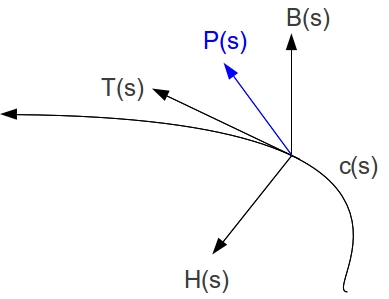
\includegraphics[scale=0.4]{Bilder/Bsp3.jpg}
\end{figure}

 \(s \mapsto c(s)\) beschreibt die Bewegung aus Punkten mit konstanter Geschwindigkeit \(w = |c'| = 1\). Die Bewegung aus starr mit der Begleitbasis \((T_1,T_2,T_3) = (T, H, B)\) verbundenen Punktes
 \[
  P(s) = c(s) + \sum_{i=1}^3 \lambda_i T_i(s) = c(s) + X(s)
 \]
setzt sich zusammen aus einer Translation\index{Translation} (mit der Kurve) und einer Drehung\index{Drehung} um eine momentane Drehachse\index{Drehung!Drehachse}. Für seine Geschwindigkeit gilt
\begin{align*}
 P'(s) &= c'(s) \sum_{i=1}^3 \lambda_i T_i' (s) = c'(s) + \sum_{i=1}^3 \lambda_i w(s) D(s) \times T_i(s) \\
 &=\uline{c'(s) + w(s) D(s) \times X(s)}
\end{align*}
mit der
\begin{itemize}
 \item (vektoriellen) Bahngeschwindigkeit\index{Geschwindigkeit!Bahn-} \(c'(s)\) der Kurve und der 
 \item (vektoriellen) Winkelgeschwindigkeit\index{Geschwindigkeit!Winkel-} \(w\cdot D)(s)\) des Vektors \(X(s) = P(s) - c(s)\) \\
 wobei \(D(s)\) der Einheitsvektor\index{Drehung!Drehachse!Einheitsvektor} der momentanen Drehachse ist \\
 und \(w(s)\)  die skalare Winkelgeschwindigkeit beschreibt
\end{itemize}

\end{kin}

\subsection{Approximierter Kurvenverlauf}
\(s \mapsto c(s)\) sei Bogenlängenparametrisierung einer \(\C^3\)-Kurve mit \(\kappa > 0\). Um einen Parameterwert \(s_0\) (ohne Einschränkung sei \(s_0 = 0\)) besitzt sie die Taylorentwicklung
\[
 c(s) = c(0) + c'(0) s + \frac12 c''(0) s^2 + \frac16 c'''(0) s^3 + \mathcal O(s^3)
\]
Mit \(x_0:= c(0),\, T_0 := T(0), \dots,\, \kappa_0 := \kappa(0), \dots\) folgt wegen \(c' = T,\, c'' = T' = \kappa H,\, c''' = \kappa' H + \kappa (-\kappa T + \tau B)\)

\begin{satz}\label{satz136}
 Eine wendepunktfreie \(\C^3\)-Kurve in Bogenlängenparametrisierung \(s \mapsto c(s)\) im \(\IR^3\) besitzt um \(s = 0\) die Taylorentwicklung\index{Taylorentwicklung}
 \begin{align*}
  c(s) = x_0 &+ \left( s - \frac16 \kappa_0^2 s^3\right) T_0 \\
  &+ \left( \frac12 \kappa_0 s^2 + \frac16 \kappa_0' s^3 \right) H_0 \\
  &+ \left(  \frac16 \kappa_0 \tau_0 s^3\right) B_0 \\
  &+ \mathcal O(s^3)
 \end{align*}
 genannt \uline{lokale kanonische Form}\index{lokale kanonische Form} der Kurve bzgl. des kartesischen Koordinatensystems (\(x_0; T_0, H_0, B_0\)) in der Umgebung von \(s = 0\) . Berücksichtigt man nur Terme niedriger Ordnung, so verhält sie sich in Koordinaten wie
 \[
  s \mapsto \left(s, \frac12 \kappa_0 s^2, \frac16 \kappa_0 \tau_0 s^3 \right)
 \]
\end{satz}

\begin{folgerung}[aus Satz \ref{satz136}] \(\)
 \begin{enumerate}
  \item[a)] Eine Kurve im \(\IR^3\) verläuft in 1. Näherung in ihrer Tangente, in 2. Näherung in ihrer Schmiegebene. Abweichungen davon sind durch Krümmung und Torsion bestimmt.
  \item[b)] Ihre Orthogonalprojektion\index{Orthogonalprojektion}
  \begin{itemize}
   \item in die \uline{Schmiegebene} verhält sich wie eine \uline{(quadratische) Parabel}
   \item in die \uline{Normalebene} verhält sich wie eine \uline{Neil'sche Parabel}
   \item in die \uline{rektifizierende Ebene} verhält sich wie eine \uline{kubusche Parabel}
  \end{itemize}
  Skizze für \(\tau > 0\) \\
  \begin{figure}[ht]
  \begin{minipage}{5cm}
    \centering
   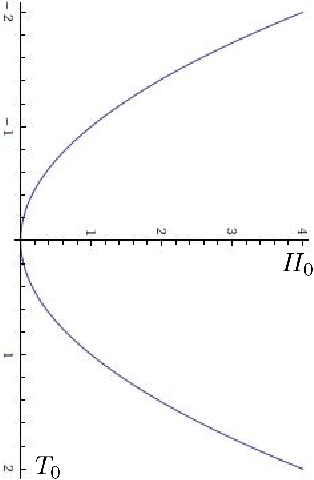
\includegraphics[scale=0.2]{Bilder/T0H0.jpg} \\
   Schmiegebene
  \end{minipage}
  \begin{minipage}{5cm}
   \centering
   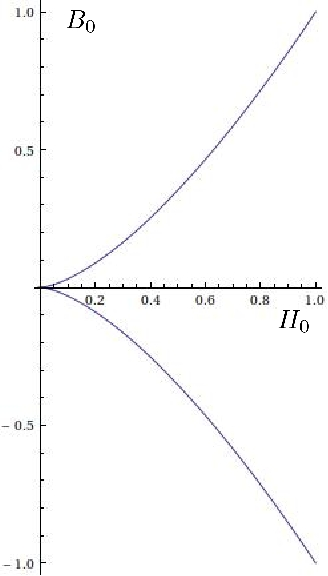
\includegraphics[scale=0.2]{Bilder/H0B0.jpg} \\
   Normalebene
  \end{minipage} 
  \begin{minipage}{5cm}
  \centering
  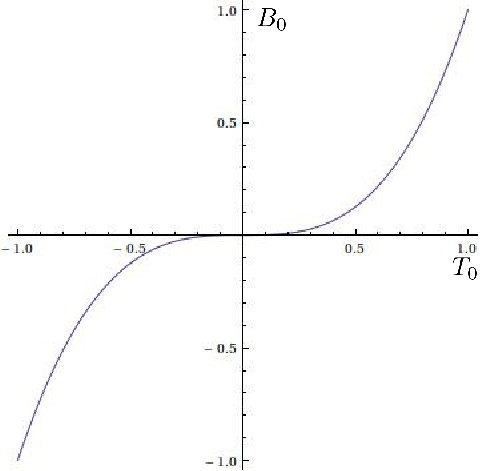
\includegraphics[scale=0.2]{Bilder/T0B0.jpg} \\
  rektifizierende Ebene
  \end{minipage}
   \end{figure} \\
   \begin{figure}[ht]
    \centering
    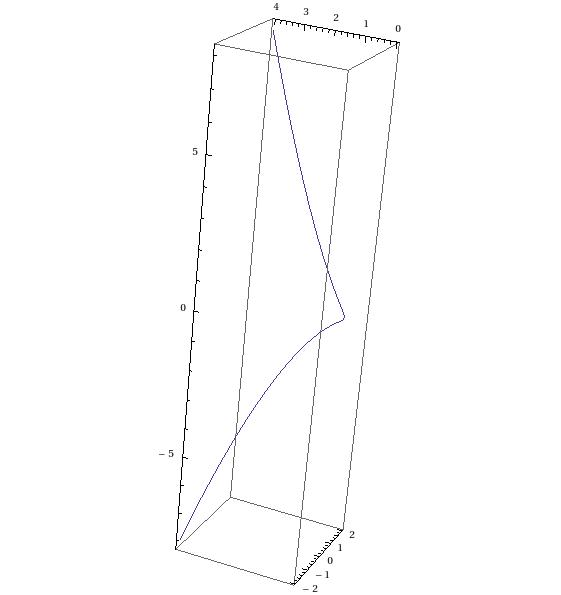
\includegraphics[scale=0.3]{Bilder/Skizze.jpg}
   \end{figure}
  \item[c)] Sie durchdringt ihre Normalebene \(x_0 + \hl H_0, B_0 \hr\) in Richtung von \(T_0\) und ihre Schmiegebene \(x_0 + \hl T_0, H_0 \hr\) für \(\uline{\tau_0 > 0}\) in Richtung von \(B_0\). (Geometrische Bedeutung des \uline{Vorzeichens der Torsion}) \\
  Sie durchdringt die rektifizierende Ebene \(x_0 + \hl B_0, T_0 \hr\) niemals, sondern bleibt auf der Seite, in die \(H_0\) zeigt.
 \end{enumerate}
\end{folgerung}

\subsection{Krümmungskreis und Schmiegkugel (oskulierende Kugel)}\index{Krümmungskreis}\index{Schmiegkugel}
Wir bestimmen alle Kugeln \(K_r(m) = \{ y \in \IR^3 \mid |y-m| = r \}\), die eine vorgegebene Kurve in Bogenlängenparametrisierung \(s \mapsto c(s)\) in einem Punkt \(c(s_0)\) von 2. und 3. Ordnung \uline{berühren}. \\\\
\uline{Berührbedingungen}\index{Berührbedingung} an die Abstandsfunktion \(s \mapsto F(s) := \dd^2 (s) = |c(s) - m|^2\)
\begin{align*}
 F(s_0) &= r^2 &\big(\text{Berührung 0. Ordnung: }c(s_0) \in K_r(m)\big) \\
 \text{zusätzlich } F'(s_0) &= 0 &(\text{Berührung 1. Ordnung}) \\
 \text{zusätzlich } F''(s_0) &= 0 &(\text{Berührung 2. Ordnung}) \\
 \text{zusätzlich } F'''(s_0) &= 0 &(\text{Berührung 3. Ordnung})
\end{align*}

\begin{begruendung} \(\)
\begin{itemize}
 \item Berührung 1. Ordnung \(=\) "`2-punktige Berührung"' 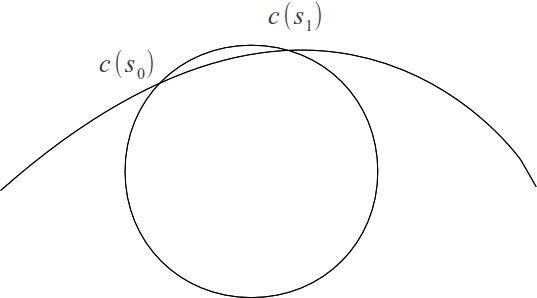
\includegraphics[scale=0.2]{Bilder/Bsp5.jpg} \\
 \(F(s_0) = F(s_1) = r^2 \stackrel{\text{MWS}}{\Rightarrow} \exists_{\overline {s_0} \in \overline{s_0 s_1}} F'(\overline{s_0}) = 0 \) \\
 Grenzübergang \(s_1 \to s_0 (\Rightarrow \overline {s_0} \to s_0)\) liefert \(F'(s_0) = 0\)
 \item Berührung 2. Ordnung \(=\)"`3-punktige Berührung"' \\
 \(F(s_0) = F(s_1) = F(s_2) = r^2 \stackrel{\text{MWS}}{\Rightarrow} \exists_{\overline{s_0}, \overline{s_1}} F'(\overline{s_0}) = F'(\overline{s_1}) = 0 \stackrel{\text{MWS}}{\Rightarrow} \exists_{\overline{\overline{s_0}}} F''(\overline{\overline{s_0}}) = 0\).\\
 Grenzübergang \(s_1, s_2 \to s_0 (\Rightarrow \overline{s_1}, \overline{\overline{s_0}} \to s_0)\) liefert \(F'(s_0) = F''(s_0) = 0\)
\end{itemize}
\end{begruendung}

\uline{Auswertung der Bedingungen}: 
\begin{enumerate}
 \item[(0)] \(F(s_0) = | c(s) - m|^2 = r^2\)
 \item[(1)] \(F'(s_0) = 2 \langle c-m, T \rangle (s_0) = 0\)
 \item[(2)] \(F''(s_0) = 2 \big[ 1 + \kappa \langle c-m, H\rangle \big] (s_0) = 0\)
 \item[(3)] \(F'''(s_0) = 2 \big[ \kappa' \langle c-m, H\rangle + \kappa \langle c-m, -\kappa T + \tau B\rangle \big](s_0) = 0\)
\end{enumerate}

Der Ansatz \(m = c(s_0) + \alpha T(s_0) + \beta H(s_0) + \gamma B(s_0)\) liefert
\begin{align*}
 \alpha &= - \langle c-m, T \rangle(s_0) \\
 \beta &= -\langle c-m, H \rangle(s_0) \\
 \gamma &= -\langle c-m, B\rangle (s_0)
\end{align*}
\begin{enumerate}
 \item[(0)] \(\alpha^2 + \beta^2 + \gamma^2 = r^2\)
 \item[(1)] \(\Rightarrow\) \({\color{red}\alpha = 0}\)
 \item[(2)] \(\Rightarrow\) \({\color{red}\beta = \frac1{\kappa(s_0)}} = \varrho(s_0) > 0\) (falls \(\kappa(s_0) > 0\))
 \item[(3)] \((\kappa' \varrho + \kappa \tau \gamma)(s_0) = 0\) \(\Rightarrow\) \({\color{red}\gamma = - \frac{\kappa'}{\kappa^2 \tau}(s_0) = \frac{\varrho'}{\tau}(s_0)}\) \big[falls \(\tau(s_0) \ne 0\)\big]
\end{enumerate}

\begin{satz}\label{satz137}\(\)
\begin{figure}[ht]
 \centering
 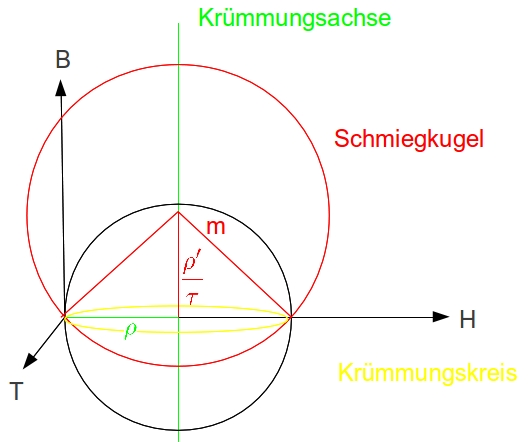
\includegraphics[scale=0.4]{Bilder/Bsp6.jpg}
\end{figure}
\begin{enumerate}
 \item Bei einer \(\C^2\)-Kurve in Bogenlängenparametrisierung \(s \mapsto c(s)\) existiert in einem Nicht-Wendepunkt \(c(s_0)\) (mit \(\kappa(s_0) > 0\)) genau eine 1-parametrige Kugelschar, die dort von 2. Ordnung berührt. Die Mittelpunkte dieser Kugel liegen auf einer Geraden
 \[
  c(s_0) + \varrho(s_0) H(s_0) + \hl B(s_0) \hr \quad \left(\text{mit } \varrho := \frac1{\kappa}\right)
 \]
 genannt \uline{Krümmungsachse}\index{Krümmungsachse} der Kurve in \(c(s_0)\). \\
 Alle diese Kugeln schneiden die Schmiegebene in einem Kreis mit Mittelpunkt 
 \[\overline m = c(s_0) + \varrho (s_0) H(s_0)\] 
 und Radius \[\overline r = \varrho(s_0)\quad \big[\text{\uline{Krümmungsradius}}\big]\]
 \index{Krümmungsradius} genannt \uline{Krümmungskreis}\index{Krümmungskreis} der Kurve in \(s_0\).
 \item Bei einer \(\C^3\)-Kurve in Bogenlängenparametrisierung \(s \mapsto c(s)\) existiert in einem Nicht-Henkelpunkt \(c(s_0)\) (mit \(\kappa(s_0) > 0, \tau(s_0) \ne 0\)) genau eine Kugel, die dort \uline{von 3. Ordnung} berührt. Sie besitzt den Mittelpunkt
 \[
  m = c(s_0) + \varrho(s_0) H(s_0) + \frac{\varrho'}{\tau}(s_0) B(s_0)
 \]
 und den Radius
 \[
  r = \sqrt{\varrho^2 + \left(\frac{\varrho'}{\tau}\right)^2}(s_0)
 \]
und heißt Schmiegkugel\index{Schmiegkugel} der Kurve in \(c(s_0)\).
\end{enumerate}
\end{satz}

\subsection{Der Fundamentalsatz der Kurventheorie (im $\IR^3$)}
\uline{Vorbemerkung}: Frenet-Theorie ist grundsätzlich nur möglich für wendepunktfreie Kurven (\(\kappa > 0\)). \\
\begin{center}
\begin{tabular}{c|c}
 \textbf{Ausreichende Differentiationsordnung} & \textbf{aber auch möglich} \\
 \begin{tabular}{c c c}
 \(c\) & \(\C^3\) &(vorausgesetzt) \\
 \hline
 \(T\) & \(\C^2\) &\\
 \(H\) & \(\C^1\) &\\
 \(B\) & \(\C^1\) &\\
 \hline
 \(\kappa\) & \(\C^1\) &\\
 \(\tau\) & \(\C^0\) &
 \end{tabular}
 &
 \begin{tabular}{c c c}
 \(c\) & \(\C^2\) &(vorausgesetzt)\\
 \hline
 \(T\) & \(\C^1\) &\\
 \(H\) & \(\C^1\) &(zusätzlich vorausgesetzt) \\
 \(B\) & \(\C^1\) &\\
 \hline
 \(\kappa\) & \(\C^0\) &\\
 \(\tau\) & \(\C^0\) &
 \end{tabular}
\end{tabular}
\end{center} 
Schon für solche "`\(\C^2\)-Kurven mit \(\C^1\)-Begleitbasis"' ("`Frenet-Kurven"') lässt sich beweisen:

\begin{satz}[Fundamentalsatz der Kurventheorie im euklidischen $\IR^3\)]\label{satz138}\index{Fundamentalsatz} \(\)
 \begin{enumerate}
  \item[a)]Seien \(s \in I \mapsto \kappa(s) > 0, \, s \in I \mapsto \tau(s) \in \IR\) beliebige \(\C^0\)-Funktionen, \(s_0 \in I\) ein Parameterwert, \(x_0 \in \IR^3\) ein Punkt und \((T_0, H_0, B_0)\) eine positiv orientierte Orthonormalbasis des \(\IR^3\). Dann gibt es genau eine \(\C^2\)-Kurve in Bogenlängenparametrisierung \(s \in I \mapsto c(s) \in \IR^3\) mit \(\C^1\)-Begleitbasis \(s \mapsto (T, H, B)(s)\), welche die Krümmung \(s \mapsto \kappa(s)\) und die Torsion \(s \mapsto \tau(s)\) besitzt, sowie die Anfangsbedingungen
  \begin{align*}
   c(s_0) = x_0, \, (T, H, B)(s_0) = (T_0, H_0, B_0) \tag{\(\ast\)}
  \end{align*}
  erfüllt.
  \item[b)] Zwei \(\C^2\)-Kurven in Bogenlängenparametrisierung \(s \mapsto c(s), \, s \mapsto \widetilde c(s)\) mit \(\C^1\)-Begleitbasis mit gleicher Krümmung \(s \mapsto \kappa(s) = \widetilde \kappa(s)\) und Torsion \(s \mapsto \tau(s) = \widetilde \tau(s)\) besitzen, stimmen überein bis auf eine (eigentliche) Bewegung (Drehung + Translation) des \(\IR^3\), d.h. es gilt
  \[
   \widetilde c = D c + t
  \]
  mit einer Drehmatrix \(D \in SO(3,\IR)\) und einem Translationsvektor \(t \in \IR^3\).
 \end{enumerate}
\end{satz}

\begin{beweis}[von Satz \ref{satz138}] \(\)
 \begin{enumerate}
  \item[a)] \textbf{\uline{Eindeutigkeit}:} Das \uline{lineare} Differentialgleichungssystem der Frenet-Formeln
  \begin{align*}
   c' = T_1, \quad \vxyz{T_1}{T_2}{T_3}' = \begin{pmatrix}
                            0 & \kappa & 0 \\
                            -\kappa & 0 &\tau \\
                            0 & -\tau & 0
                           \end{pmatrix} \vxyz{T_1}{T_2}{T_3} \text{ bzw. } T_i' = \sum_{k = 1}^3 a_{ik} T_k
  \end{align*}
  besitzt zu den Anfangsbedingungen \((\ast)\) \big(bzw. hier \((T_1, T_2, T_3)(s_0) = (T_0, H_0, B_0)\)\big) \uline{genau eine} \(\C^1\)-Lösung \[s \mapsto (T_1, T_2, T_3)(s_0)\] und damit genau eine \(\C^2\)-Lösung \[s \mapsto c(s) = x_0 + \int_{s_0}^s T_1(\sigma) \dd \sigma\], definiert \uline{auf ganz \(I\)}. \\\\
  \textbf{\uline{Existenz}}: Es muss noch überprüft werden, ob diese Lösung \(s \mapsto c(s)\) Bogenlängen\-para\-metri\-sierung einer \uline{\(\C^2\)-Kurve} mit \(\C^1\)-Begleitbasis ist und wirklich \(s \mapsto \kappa(s), \tau(s)\) als Krümmung und Torsion besitzt.
  \begin{enumerate}
  \item[\((\alpha)\)] Wir zeigen: Die Lösungsfelder \(s \mapsto T_1(s), T_2(s), T_3(s)\) bilden \uline{überall} (nicht nur für \(s = s_0\)) eine positiv orientierte Orthonormalbasis: \\
  Für die Skalarprodukte \(\langle T_i, T_k \rangle\) gilt:
  \begin{align*}
   \uline{\langle T_i, T_k \rangle'} = \langle T_i', T_k \rangle + \langle T_i, T_k' \rangle = \sum_{j = 1}^3 a_{ij} \uline{\langle T_j, T_k \rangle} + \sum_{k=1}^3 a_{kj} \uline{\langle T_i, T_j \rangle}
  \end{align*}
  Dieses \uline{lineare} Differentialgleichungssystem besitzt zu den Anfangsbedingungen \[\langle T_i, T_k \rangle(s_0) = \delta_{ik}\] \uline{genau eine} Lösung und diese ist \(\langle T_i, T_k \rangle \equiv \delta_{ik}\), denn
  \begin{align*}
   0 = \delta_{ik}' = a_{ik} + a_{ki}
  \end{align*}
  weil die Ableitungsmatrix schiefsymmetrisch ist. \\
  Weiter muss für das Orthonormalbasisfeld \(s \mapsto (T_1, T_2, T_3)(s)\) gelten: \[\det(T_1, T_2, T_3) = \pm 1\], wobei aus Stetigkeitsgründen nur \(+1\) möglich ist \big(denn \(\det(T_1, T_2, T_3)(s_0) = +1\)\big).
  \item[\((\beta)\)] Für die Lösung \(s \mapsto c(s)\) gilt jetzt \(|c'| = |T_1| = 1\), d.h. sie ist Bogen\-längen\-para\-metri\-sierung einer \uline{Kurve} im \(\IR^3\). Weiter ist
  \begin{align*}
   T &= c' = T_1 \\
   H &= \frac{T'}{|T'|} = \frac{T_1'}{|T_1'|} = \frac{\kappa T_2}{\kappa |T_2|} = T_2 \\
   B &= T \times H = T_1 \times T_2 = T_3
  \end{align*}
  Es gelten also die Frenet-Formeln für \((T, H, B)\), sodass \(\kappa\) die Krümmung und \(\tau\) die Torsion ist.
  \end{enumerate}
 \item[b)] Sei \(s_0\) ein fester Parameterwert sowie 
 \begin{align*}
  x_0 &:= c(s_0) \\
  (T_0, H_0, B_0) &:= (T, H, B)(s_0) \\
  \widetilde{x}_0 &:= \widetilde c(s_0) \\
  \left(\widetilde T_0, \widetilde H_0, \widetilde B_0 \right) &:= \left(\widetilde T, \widetilde H, \widetilde B\right)(s_0)
 \end{align*}
 Dann gibt es genau eine Drehmatrix \(D\) und einen Vektor \(t \in \IR^3\) mit
 \begin{align*}
  \widetilde x_0 &= D x_0 + t \\
  \widetilde T_0 &= D \cdot T_0 \\
  \widetilde H_0 &= D \cdot H_0 \\
  \widetilde B_0 &= D \cdot B_0
 \end{align*}
 (Transformation zweier kartesischer Koordinatensysteme ineinander). \\
 Das lineare Differentialgleichungssystem
 \[
  c' = T_1, \quad \vxyz{T_1}{T_2}{T_3}' = \begin{pmatrix}
                                           0 & \kappa & 0 \\
                                           -\kappa & 0 & \tau \\
                                           0 & -\tau & 0
                                          \end{pmatrix} \vxyz{T_1}{T_2}{T_3}
 \]
 hat nun die Lösungssysteme
 \begin{enumerate}
  \item[(1)] \(s \mapsto c(s), \quad s \mapsto (T, H, B)(s_0)\)
  \end{enumerate}
  und wegen er Linearität
  \begin{enumerate}
  \item[(1a)] \(s \mapsto D \cdot c(s) + t, \quad s \mapsto (D \cdot T, D \cdot H, D \cdot B)\)
  \end{enumerate}
  sowie natürlich auch
  \begin{enumerate}
  \item[(2)] \(s \mapsto \widetilde c(s), \quad s \mapsto \left(\widetilde T, \widetilde H, \widetilde B\right)(s)\) \\
 \end{enumerate}
 wobei (1a) und (2) in \(s_0\) die gleichen Anfangsbedingungen besitzen
 \[
  \widetilde c(s_0) = \widetilde x_0 = D x_0 + t, \dots
 \]
Also gilt identisch
\begin{align*}
 \widetilde c &= D \cdot c + t \\
 \text{und } \left(\widetilde T, \widetilde H, \widetilde B\right) &= (D \cdot T, D \cdot H, D \cdot B)
\end{align*}

 \end{enumerate}
\end{beweis}

\textbf{Ergebnis}: Krümmung und Torsion als Funktionen der Bogenlänge bilden ein \uline{vollständiges} Sys\-tem \uline{unabhängiger} Invarianten für eine Frenet-Kurve im \(\IR^3\).

\begin{bemerkung}
 Das Differentialgleichungssystem der Frenet-Formeln lässt sich nur in einfachen Fällen explizit lösen, etwa bei ebenen Kurven als Spezialfälle von Böschungslinien.
\end{bemerkung}

\begin{variante}[des Fundamentalsatzes]
 Vorgabe von \[\begin{cases}
                t \mapsto w(t) > 0 & \text{(Geschwindigkeit)} \\
                t \mapsto \kappa(t) > 0 & \text{(in Abhängigkeit von der Zeit)} \\
                t \mapsto \tau(t)
               \end{cases}\]
 bestimmen eine Kurve in einer Parameterdarstellung \(t \mapsto c(t)\) mit \(|\dot c| = w\) eindeutig. Das Differentialgleichungssystem 
 \begin{align*}
  \dot c &= w T_1 \\
  \frac{\dd}{\dd t}\vxyz{T_1}{T_2}{T_3} &= w \begin{pmatrix}
                                             0 & \kappa & 0 \\
                                             -\kappa & 0 & \tau \\
                                             0 & -\tau & 0 
                                            \end{pmatrix} \vxyz{T_1}{T_2}{T_3}
 \end{align*}
 ist zu lösen.
\end{variante}

\subsection{Spezielle Kurvenklassen}
\subsubsection{A. Böschungslinien}

\begin{definition}
 Eine Böschungslinie\index{Böschungslinie} im \(\IR^3\) ist eine \(\C^1\)-Kurve, ohne Einschränkung in Bogenlängenparametrisierung \(s \mapsto c(s)\), deren Tangenten mit einer \uline{festen Richtung} \(E\) (mit \(|E| = 1\)) einen festen \uline{Böschungswinkel}\index{Böschungswinkel} \(\gamma\) einschließen. Es ist also \(\forall_s\)
 \[
  \langle T(s), E \rangle = \cos \gamma
 \]
\end{definition}

\begin{bsp}\(\)
 \begin{enumerate}
  \item Ebene Kurven (\(\gamma = 90^{\circ}\))
  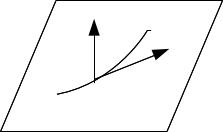
\includegraphics[scale=0.2]{Bilder/ebene_kurve.jpg}
  \item Gewöhnliche Schraubenlinien
  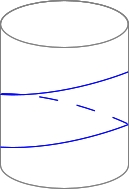
\includegraphics[scale=0.2]{Bilder/schraube.jpg}
 \end{enumerate}
\end{bsp}

\begin{bemerkung}
 Bei \uline{Frenet-Böschungslinien} folgt aus \(\langle T, E \rangle = \const.\) sofort \(\kappa \langle H, E \rangle = 0\), sodass \(E\) in der rektifizierenden Ebene \(c + \hl T, B \hr\) liegt. Der Böschungswinkel \(\gamma\) kann dann eindeutig so festgelegt werden, dass
 \begin{align*}
  E = \cos \gamma \, T + \sin \gamma \, B \quad \text{mit } -\pi < \gamma \le \pi \tag{\(\ast\)}
 \end{align*}
Durch Übergang von \(E\) zu \(-E\) bei Bedarf kann erreicht werden, dass \(\sin \gamma = \langle E, B \rangle \ge 0\), also \(\uline{0 \le \gamma \le \pi}\). Ableiten von \((\ast)\) liefert
\begin{align*}
 0 = (\kappa \cos \gamma - \tau \sin \gamma) \cdot H, \quad \text{also } \uline{\kappa \cos \gamma - \tau \sin \gamma = 0}
\end{align*}
sodass nur \(\uline{0 < \gamma < \pi}\) möglich ist.
\end{bemerkung}

\begin{satz}\label{satz139}
 Für eine Frenet-Kurve im \(\IR^3\) sind äquivalent
 \begin{enumerate}
  \item[(a)] Die Kurve ist Böschungslinie. \big(\(\langle T, E\rangle = \const.\)\big)
  \item[(b)] Die \uline{konische Krümmung}\index{Krümmung!konische} \mat{\frac{\tau}{\kappa} (= \varrho \tau)} ist konstant.
  \item[(c)] Der Darboux-Vektor \mat{D = \frac1\omega (\tau T + \kappa B)} ist konstant \big[und ohne Einschränkung gleich der festen Richtung\big]
  \item[(d)] Der Winkel zwischen Tangentenrichtung und Darboux-Richtung ist konstant: \(\uline{\langle T, D \rangle = \const}\) \big[und ohne Einschränkung gleich dem Böschungswinkel\big]
 \end{enumerate}
\end{satz}

\begin{beweis}[von Satz \ref{satz139}] \(\)
\begin{enumerate}
 \item[(a) \(\Rightarrow\) (b)] Nach obiger Bemerkung gilt
 \begin{align*}
  &\kappa \cos \gamma - \tau \sin \gamma = 0 \\
  &\Rightarrow \frac{\tau}{\kappa} = \cot \gamma = \const.
 \end{align*}
 \item[(b) \(\Rightarrow\) (c)] 
 \begin{align*}                                 
&\frac{\tau}{\kappa} = \lambda = \const. \Rightarrow \begin{cases}
                                                     \frac{\kappa}{\omega} = \frac{\kappa}{\sqrt{\kappa^2 + \tau^2}} = \frac{1}{\sqrt{1 + \lambda^2}} = \const. \\
                                                     \frac{\tau}{\omega} = \frac{\tau}{\sqrt{\kappa^2 + \tau^2}} = \frac{\lambda}{\sqrt{1 + \lambda^2}} = \const.
                                                    \end{cases} \\
&\Rightarrow D' = \left(\frac{\tau}{\omega} T + \frac{\kappa}{\omega} B\right)' = \left(\frac{\tau}{\omega} \kappa - \frac{\kappa}{\omega} \tau\right)H = 0
\end{align*}
\item[(c) \(\Rightarrow\) (d)] \(D = \const. \Rightarrow \langle T, D \rangle' = \kappa \langle H, D\rangle = 0\)
\item[(d) \(\Rightarrow\) (a)] \begin{align*}                               
&\langle T, D\rangle = \frac{\tau}{\omega} = \const. \Rightarrow \left(\frac{\kappa}{\omega}\right)^2 = 1 - \left(\frac{\tau}{\omega}\right)^2 = \const \\
&\Rightarrow \frac{\tau}{\omega}, \frac{\kappa}{\omega} = \const. \Rightarrow D' = \dots = 0 \\
&\Rightarrow D = \const. \Rightarrow \text{ Die Kurve ist Böschungslinie mit fester Richtung } E := D
                               \end{align*}
 \end{enumerate}
\end{beweis}

\subsubsection{A. Sphärische Kurven}
\begin{satz}\label{satz1310}\(\)
 \begin{enumerate}
  \item[a)] Eine wendepunktfreie \(\C^2\)-Kurve in Bogenlängenparametrisierung \(s \mapsto c(s)\) ist genau dann \uline{sphärisch}\index{sphärisch} (liegt auf einer Kugel), wenn eine \(\C^1\)-Funktion \(s \mapsto a(s)\) existiert mit
  \begin{center}\(\boxed{\begin{aligned}
   \varrho' &= a \tau \\
   a' &= -\varrho \tau
  \end{aligned}}\)\end{center}
  Für Mittelpunkt \(m\) und Radius \(r\) der Kugel gilt dann
  \[
   m = c + \varrho H + a B, \quad r = \sqrt{\varrho^2 + a^2}
  \]
  \item[b)] Äquivalent dazu ist: Es existiert eine \(\C^1\)-(Winkel)-Funktion \(s \mapsto \lambda (s)\) mit \(|\lambda| < \frac{\pi}{2}\) und eine Zahl \(r > 0\) mit \(\uline{\varrho = r \cos \lambda, \, \lambda' = -\tau}\). Dabei gilt
  \[
   m = c + r (\cos \lambda \, H + \sin \lambda \, B)
  \]
 \end{enumerate}

\end{satz}

\begin{beweis}[von Satz \ref{satz1310}] \(\)
 \begin{enumerate}
  \item[a)] 
  \begin{align*}
  &\forall_s \, |c(s) - m|^2 = r^2 \Rightarrow \forall_s \, \langle c(s) - m, T(s) \rangle = 0 \\
  &\Rightarrow c = m - b H - a B
  \end{align*}
  mit \(\C^1\)-Funktionen \(a, b\). Aus
  \begin{align*}
   T = -b' H - b (-\kappa T + \tau B) - a' B + a \tau H
  \end{align*}
  folgt durch Koeffizientenvergleich
  \begin{align*}
   b \cdot \kappa &= 1 \quad (\Rightarrow b = \varrho) \\
   b' &= a \cdot \tau \\
   a' &= -b \cdot \tau
  \end{align*}
  \uline{Rückrichtung}: Aus \(\varrho' = a \tau, \, a' = -\varrho \tau\) folgt für \(m := c + \varrho H + a B\):
  \begin{align*}
   m' = \dots = 0 \quad \text{also}\quad m = \const.
  \end{align*}
  und für \(r^2 := |c-m|^2 = \varrho^2 + a^2\) folgt:
  \begin{align*}
   \frac{\dd}{\dd s} (r^2)= 2 \varrho \varrho' + 2 a a' = 0 \quad \text{also} \quad r = \const.
  \end{align*}
  \item[b)]
  "`\(\Rightarrow\)"' Setze \(\begin{Bmatrix}
                               \rho = r \cos \lambda &(> 0)\\
                               a = r \sin \lambda
                              \end{Bmatrix}\), also \[\lambda = \arctan \frac a\varrho \in \left] -\frac{\pi}2, + \frac{\pi}2\right[ \]
Dann ist \mat{\tau = - \frac{a'}{\varrho} = -\frac{r (\cos \lambda) \lambda'}{r \cos \lambda} = -\lambda '} \par
"`\(\Leftarrow\)"' \(\dots\)
 \end{enumerate}

\end{beweis}

\begin{folgerung} \(\)
 \begin{enumerate}
  \item[a)] Sphärische \(\C^4\)-Kurven mit \(\forall_s \kappa(s) > 0, \forall_s \tau \ne 0\) sind durch
  \[
   \left(\frac{\varrho'}{\tau}\right)' + \varrho \tau = 0
  \]
  definiert.
  \item[b)] Äquivalent dazu ist, wenn zusätzlich \boxed{\text{"`verrat ich net"'}}
  \[
   \left(\frac{\varrho'}{\tau}\right)^2 + \varrho^2 = \const (= r^2)
  \]
  Die Kugel, auf der die Kurve verläuft, ist ihre Schmiegkugel.
 \end{enumerate}
\end{folgerung}

\begin{beweis}[der Folgerung] \(\)
 \begin{enumerate}
  \item[a)] Elimination von \(a\)
  \item[b)] siehe Übungen
 \end{enumerate}

\end{beweis}

\section{Kurven im euklidischen $\IR^n$}
Hier ist Frenet-Theorie möglich für \(\C^n\)-Kurven, ohne Einschränkung in Bogenlängenparametrisierung \(s \mapsto c(s)\), deren Schmieghyperebenen
\[
 S_{n-1} = c + \hl c_1, \dots, c_{n-1} \hr \quad \left(\text{mit } c_p := \frac{\dd^p c}{\dd s^p}\right)
\]
nirgends degenerieren, also überall \((c_1, \dots, c_{n-1})\) linear unabhängig ist.

\textbf{\uline{Begleitbasis}:} \\
Anwendung des Schmidt'schen Orthonormalisierungsverfahrens auf die Basis \((c_1, \dots, c_{n-1})\) der Schmieghyperebene liefert dort eine Orthonormalbasis \((T_1, \dots, T_{n-1})\), die durch \(T_n := T_1 \times \dots \times T_{n-1}\) zu einer positiv orientierten, orthonormierten Begleitbasis \((T_1, \dots, T_n)\) der Kurve ergänzt werden kann. \par
\textbf{\uline{Ableitungsgleichungen}:}\index{Ableitungsmatrix!$\IR^n$} \\
Aus \(\langle T_i, T_k\rangle = \delta_{ik} \Rightarrow \langle T_i', T_k\rangle = -\langle T_k', T_i \rangle\) folgt die Schiefsymmetrie der Ableitungsmatrix \[\left( \langle T_i', T_k\rangle \right)_{i,k = 1, \dots, n}\]
Wegen 
\begin{align*}
T_p \in \hl c_1, \dots, c_p \hr \Rightarrow T_p' &\in \hl c_1, \dots, c_{p+1} \hr \\
&= \hl T_1, \dots, T_{p+1}\hr
\end{align*}
für \(\forall_{q > p+1} \langle T_p', T_q\rangle = 0\). \par
So folgt nun der Satz:

\begin{satz}\label{satz141}
 Sei \(s \mapsto c(s)\) Bogenlängenparametrisierung einer \(\C^n\)-Kurve im \(\IR^n\) mit \(\forall_s \big(c_1, \dots, c_{n-1}\big)(s)\) linear unabhängig. Dann genügt die durch
 \begin{align*}
  T_1 &:= c' \\
  \overset{n-2}{\underset{p=1}\forall} \, T_{p+1} &:= \frac{c_{p+1} - \sum_{k=1}^p \langle c_{p+1}, T_k\rangle T_k}{| \dots |} = \frac{[c_{p+1}]_\perp}{\left|[c_{p+1}]_\perp\right|} \\
  T_n &:= T_1 \times \dots \times T_{n-1}
 \end{align*}
rekursiv definierte \uline{Frenet-Begleitbasis} \(s \mapsto \big(T_1, \dots, T_n\big)(s)\) den Ableitungsgleichungen
\[
 \begin{pmatrix}
  T_1 \\
  \vdots \\
  \vdots \\
		\vdots \\
		\vdots \\
  T_n
 \end{pmatrix}' =
 \begin{pmatrix}
 0          & \kappa_1  & 0        & \hdots        & \hdots       & 0 \\
 -\kappa_1  & 0         & \kappa_2 & \ddots        &              & \vdots \\
 0          & -\kappa_2 &   \ddots & \ddots        & \ddots       & \vdots \\
 \vdots     & \ddots    & \ddots   & \ddots        & \kappa_{n-2} & 0 \\ 
 \vdots     &           & \ddots   & -\kappa_{n-2} & \ddots       & \tau\\
 0          & \hdots    & \hdots   & 0             & -\tau        & 0 
\end{pmatrix} \begin{pmatrix}
		T_1 \\
		\vdots \\
		\vdots \\
		\vdots \\
		\vdots \\
		T_n
	      \end{pmatrix}
\]
mit den \(n-2\) \uline{Krümmungen}
\[
 s \mapsto \kappa_p (s) = \langle T_p', T_{p+1} \rangle (s) \quad (p = 1, \dots, n-2)
\]
und der \uline{Torsion}
\[
 s \mapsto \tau(s) = \langle T_{n-1}', T_n \rangle(s)
\]
\uline{Zusatz}: \\
Es gilt auch
\begin{align*}
 \kappa_p &= \left| [T_p']_\perp \right| = \left| T_p' - \sum_{k=1}^p \langle T_p', T_k\rangle T_k \right| > 0 \quad (p = 1, \dots, n-2) \\
 \tau &= \det(T_1, \dots, T_{n-1}, T_{n-1}') \gtreqqless 0
\end{align*}

\end{satz}

\begin{beweis}[des Zusatzes] \(\)
 \begin{enumerate}
  \item Es ist 
  \begin{align*}
  T_p = \lambda \left(c_p + \sum_{k=1}^{p-1} \lambda_k c_k\right) = [c_p]_\perp \text{ mit } \lambda = \frac{1}{|[c_p]_\perp|} > 0
  \end{align*}
  also
  \[
   T_p' = \lambda c_{p+1} + \sum_{k=1}^p \widetilde{\lambda}_k c_k \Rightarrow \uline{[T_p']_\perp = \lambda [c_{p+1}]_\perp}
  \]
  Ebenso ist
  \[
   \uline{T_{p+1} = \mu [c_{p+1}]_\perp} \text{ mit } \mu = \frac{1}{|[c_{p+1}]_\perp|} > 0
  \]
  Es folgt
  \begin{align*}
   \kappa_p &= \langle T_p', T_{p+1} \rangle = \langle [T_p']_\perp, T_{p+1}\rangle \\
   &= \lambda \cdot \mu |[c_{p+1}]_\perp |^2 = \uline{\frac{|[c_{p+1}]_\perp|}{|[c_p]_\perp|} = [T_p']_\perp} > 0
  \end{align*}
  \item \(\tau = \langle T_{n-1}', T_n \rangle = \langle T_1 \times \dots \times T_{n-1}, T_{n-1}' \rangle = \det ( T_1, \dots, T_{n-1}, T_{n-1}')\)
 \end{enumerate}

\end{beweis}

\uline{Geometrische Bedeutung}
 \begin{itemize}
  \item der Krümmung \(\kappa_p\): Abweichung vom Verlauf in der Schmiegebene \(S_p\)
  \item der Torsion \(\tau\): Abweichung vom Verlauf in der Schmieghyperebene \(S_{n-1}\) \uline{mit Orientierung! (Vorzeichen)} 
 \end{itemize}

\begin{satz}[Fundamentalsatz]\label{satz142}\index{Fundamentalsatz}
\[\kappa_1, \ldots, \kappa_{n-2}, \tau\] 
als Funktionen der Bogenlängen bilden ein \uline{vollständiges} System  \uline{unabhängiger} Invarianten.
\end{satz}
Berechnung der Größen bezüglich einer beliebigen Parametrisierung:
\begin{folgerung}
Bezüglich einer beliebigen, zulässigen Parametrisierung \(t \mapsto c(t)\) einer Frenet-Kurve im \(\IR^n\) gilt mit \(c_p:=\frac{\dd^p c}{\dd t^p} (p=1, \dots , n)\)
\begin{align*}
 T_1 &=\frac{c_1}{|c_1|} \\
 \overset{n-2}{\underset{p=1}{\forall}} T_{p+1} &= \frac{c_{p+1} - \sum_{k=1}^p \langle c_{p+1}, T_k \rangle T_k}{| \dots |} = \frac{[c_{p+1}]_{\perp}}{\left| [c_{p+1}]_{\perp} \right|} \\
 T_n &= T_1 \times \ldots \times T_{n-1}
\end{align*}
sowie mit
\begin{align*}
 A_0 &:= 1\\
 A_p &:= a_p \left(c_1, \ldots , c_p \right) = \sqrt{\det \left( \langle c_i, c_k \rangle \right)_{i,k = 1, \l[c_{p+1}]_{\perp}dots , p}} > 0 \quad (p = 1, \ldots, n-1)\\
 V_n &:= \det \left(c_1, \ldots , c_n \right) \gtreqqless 0\\
 \overset{n-2}{\underset{p=1}{\forall}} \kappa_p &= \frac{1}{|\dot c|} \frac{A_{p+1}}{A_p} \left/\frac{A_p}{A_{p-1}}\right.  > 0\\
 \tau &= \frac{1}{|\dot c|} \frac{V_n}{A_{n-1}}\left/\frac{A_{n-1}}{A_{n-2}} \right. \gtreqqless 0
\end{align*}
\end{folgerung}
\textbf{Spezialfälle:}\\
\begin{align*}
\uline{n=2:}\quad \tau &= k = \frac{1}{|\dot c|} \frac{V_2}{A_1}\left/\frac{A_1}{A_0}\right. = \frac{\det(\dot c, \ddot c)}{|\dot c|^3} \quad \big(A_1 = |\dot c|, V_2 = \det (\dot c, \ddot c)\big) \\
\uline{n=3:}\quad \kappa &= \frac{1}{|\dot c|} \frac{A_2}{A_1}\left/\frac{A_1}{A_0} \right. = \frac{a_2 (\dot c, \ddot c)}{|\dot c|^3} = \frac{|\dot c, \times \ddot c|}{|\dot c|^3} \\
\tau &= \frac{1}{|\dot c|} \frac{V_3}{A_2}\left/\frac{A_2}{A_1} \right. = \frac{\det (\dot c, \ddot c, \dddot c)}{|\dot c\times \ddot c|^2} 
\end{align*}
\begin{beweis}[Beweisskizze zu Satz \ref{satz142}]
Darstellung von \(T_1, \ldots T_n \) klar, da das Orthonormalisierungsverfahren unabhängig von der Ausgangsbasis ist, wenn \( \hl c_1, \ldots , c_p \hr = \hl \widetilde c_1, \dots \widetilde c_p \hr\) samt Orientierung
\begin{align*}
 \kappa_p = \langle T'_p, T_{p+1} \rangle = \frac{1}{w} \langle \dot T_p, T_{p+1} \rangle \stackrel{\ast}{=} \frac{1}{w} \frac{|\left[c_{p+1} \right]_\perp|}{|\left[c_p \right]_\perp|}\\
 \ast = \text{siehe Beweis des Zusatzes}
\end{align*}
Nach der Formel "`Volumen \(=\) Grundfläche \(\times\) Höhe"' gilt
\begin{align*}
  a_{p+1} (c_1, \dots , c_{p+1}) &= a_p \left(c_1, \dots , c_p \right) \cdot \left|\left[c_{p+1}\right]_\perp\right| \text{, also } \\
  \left|\left[c_{p+1}\right]_\perp\right| &= \frac{A_{p+1}}{A_p}
\end{align*}
\end{beweis}